%% This is an example first chapter.  You should put chapter/appendix that you
%% write into a separate file, and add a line \include{yourfilename} to
%% main.tex, where `yourfilename.tex' is the name of the chapter/appendix file.
%% You can process specific files by typing their names in at the 
%% \files=
%% prompt when you run the file main.tex through LaTeX.
\chapter{{\em Silhouette} Execution}
This chapter introduces {\em silhouette} 
execution as a possible solution to the bootstorm
problem (Section \ref{def:sil}).
It then explains the dynamic instrumentation 
techniques we used to simulate and improve silhouette execution
for concurrently booting VMs (Section \ref{silsimulation}). Finally,
it evaluates the effectiveness
of silhouette execution in solving the 
bootstorm problem (Section \ref{sileval}). 

\section{What is {\em Silhouette} execution?} \label{def:sil}
{\em Silhouette} execution encapsulates the 
novel design idea that information recorded from one
execution of a program can be used to 
bypass execution steps of subsequent instances
of the same program. Precise knowledge
of where program execution can diverge 
is indispensable to such a design.
Silhouette execution is designed
extend CPU capabilities much like
memory overcommitment is designed to extend
the memory resources of host machines.
One possible design that employs silhouette execution
to save on CPU usage from 
running the same program multiple times is as follows:

\begin{itemize}
\item We run one program instance -- the {\em leader} -- before
we all others.
\item Using information collected from the {\em leader} (e.g.
via dynamic instrumentation techniques), 
we precisely identify instructions where
other instances of the program could diverge.
We call these instructions {\em fork-points}.
\item From the leader, we also collect an {\em execution signature} 
that summarizes its execution between successive
fork-points. For a user-space program, this could
include a record of memory operations and 
system calls.
\item We do not execute all instructions from execution
instances -- or {\em silhouettes} -- that are run
after the leader. Instead, each silhouette skips execution to
the next fork-point by executing memory
operations and system-calls before that fork-point. 
It then executes the {\em forking} instruction.
\item If a forking instruction
in a silhouette has different side-effects from
the corresponding instruction in the leader, 
the silhouette branches execution and continues
executing instructions of its own. 
Otherwise, the silhouette bypasses
execution to the next fork-point by
executing only memory operations and
system calls before the next fork-point.
\end{itemize}

The description above describes how silhouette execution
could be used to save on CPU usage from running
the same user-space program across multiple concurrently
booting VMs. 
This design can be further generalized to the execution of entire
VMs themselves, but then our definitions of fork-points
and execution signatures would have to account nondeterminism that can
arise from all software layers inside a VM.
We focus on the design of 
using silhouette execution on user-space programs as 
a first step: after all, as outlined
Section \ref{linuxboot}, concurrently booting VMs
can saturate host CPUs when they launch many
common user-space processes. 

The fundamental -- and significant -- difference
between silhouette execution and record-and-replay
approaches is that silhouette execution
does not semantically alter the executions
of silhouettes by making them blindly following
the leader. Instead, silhouettes exploit commonality 
between multiple concurrent executions to reduce CPU 
overhead. Silhouettes are faithful executions of a program
in user-space that can semantically branch from the 
leader's execution at any point because we execute all system calls
on behalf of silhouettes rather than simply emulating them
like record-and-replay approaches.

Several specific metrics are important in
evaluating the feasibility of silhouette
execution for the bootstorm scenario:
\begin{itemize}
\item Ideally, delaying the first fork-point
to be as late into silhouette execution as possible
would {\em guarantee} that we avoid
executing many redundant instructions and
save on CPU usage.
\item More generally, having few
fork-points is desirable because it reduces
the design complexity and overhead associated with 
figuring out whether a silhouette has diverged
in execution from a leader or not.
\item Having fork-points that are
separated by very many instructions
can help compress execution logs.
For instance, we could forget intermediate
values of memory locations and only
remember their final values instead.
\item Finally, programs that have a high
ratio of user-mode instructions to system-calls
and memory operations would clearly 
improve the savings from silhouette execution.
\end{itemize}

\section{Simulation Scheme} \label{silsimulation}
We modified our data collection scheme from Chapter \ref{ch:boot} (shown in 
Figure \ref{data:naive}) to simulate and
evaluate silhouette execution in the bootstorm scenario.

\begin{figure}[]
  \center
  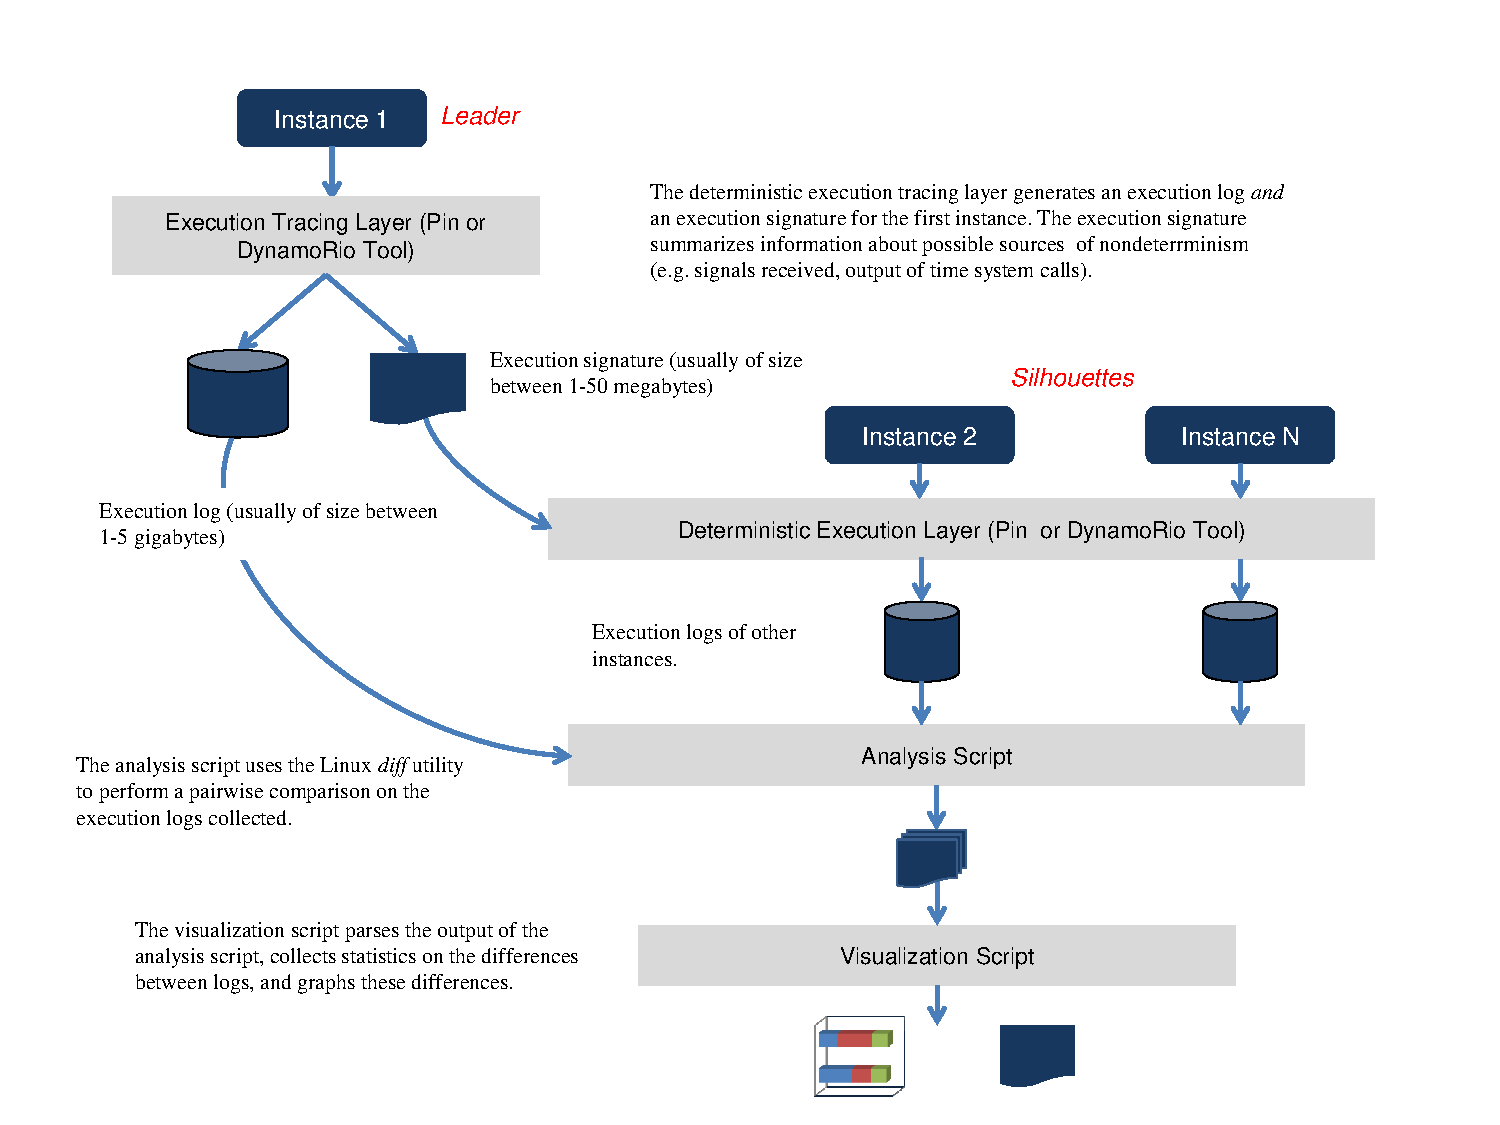
\includegraphics[scale=0.7, trim=1cm 0cm 1cm 0cm]
                  {simulation.pdf}
  \caption[Simulation of {\em Silhouette Execution} in a bootstorm scenario]%
  {Simulation of {\em Silhouette Execution} in a bootstorm scenario.
    We use dynamic instrumentation to 
    generate an execution signature file for the leader.
    While we do not bypass execution in the 
    silhouettes, try to reduce the number of fork-points 
    and record information about them.
    Our analysis and visualization
    scripts allow us to simualate and evaluate
    the effectiveness of {\em silhouette} execution.
  }
  \label{ch3:figsimulation}
\end{figure}

As shown by Figure \ref{ch3:figsimulation}, we run one instance of the
program -- the {\em leader} -- before all others.
For the leader, we generate an {\em execution log}, as before,
but we also augment the log by summarizing information about the sources of nondeterminism
described in Section \ref{ch3:sources}. For instance, we record
information about signal timing, process IDs, time-related system calls
in the {\em execution signature} file. Our dynamic instrumentation tool
uses the execution signature of the leader
to modify the instruction sequences executed by subsequently
executions (the {\em followers}), to boost determinism as much as possible.
Even though we use specific terminology, this simulation scheme can be
reconciled with multiple possible solutions to the 
boot storm scenario that involve:
\begin{itemize}
\item
booting one VM before others,
then using its execution trace to {\em speed-boot} other VMs
in a less hardware-intensive manner, or
\item 
running VMs concurrently but with an assigned leader;
the VMs communicate with each other to overcome
nondeterminism.
\end{itemize}

In the first case, the execution signature file
conceptually represents the trace of the first VM used to speed-boot
other VMs. In the second case, it represents a log of the communications 
sent from the leader sent to concurrently booting VMs. Possible
design ideas for the bootstorm scenario are described 
in Chapter \ref{ch:design}.

We now briefly describe how dynamic instrumentation can be used to overcome
the sources of nondeterminism described in \ref{ch3:sources}. \newline

\noindent {\bf Address Space Layout Randomization (ASLR)} \newline
Existing record-and-replay systems get around ASLR by
forcing the operating system to use the same address space layout across
different runs. A slightly more complex approach 
would use base/offset computations to translate two equivalent 
addresses between different executions. 
For our experiments, we simply disabled ASLR using the command
\texttt {sudo kernel.randomize\_va\_space=0} to simulate the 
case where we nudge the operating system to construct
similar address spaces for the same process. \newline

\noindent {\bf Canary and Pointer Guard Values} \newline
Dynamic instrumentation can be used to force canary (\texttt{gs:0x14})
and pointer guard (\texttt{gs:0x18}) values
to agree across distinct executions of the same program:
instructions that initialize them can be
modified or replaced; the \texttt{AT\_RANDOM} bytes 
provided by the kernel can be
modified before they are read by the application; 
values read from \texttt{`/dev/urandom'} can be 
intercepted and modified; the \texttt{rdtsc} instruction can be emulated.
The last three approaches are needed to control nondeterminism
from randomization anyway and suffice for our purpose. \newline

\noindent {\bf Randomization and Time} \newline
To overcome nondeterminism resulting from randomization,
we need to intercept the standard techniques
used by programs to seed PRNGs.
As already mentioned, values read from \texttt{`/dev/urandom'}
or the \texttt{rdtsc} instruction can be easily replaced
using the execution signature file for the first instance.

Time-related system calls can
be intercepted in the same manner:
the timestamps logged
in the execution signature file
can be used to force agreement
between different executions.
For most time-related system calls,
high-fidelity replay is not necessary:
several timestamps generated
during program execution are simply ignored
(e.g. from \texttt{stat} calls),
so they can actually be replaced with any 
fixed value. Many timestamps
returned from system calls are only compared to
determine ``freshness'': they
can be replaced with deterministic ordinal values (e.g 0 or 1) that 
perserve the original comparison result.

Conceptually, these approaches simulate the possible but highly
unlikely case that all the instances of the same program
executed time-related system calls
at precisely the same times,
and several randomly generated values independently agreed. \newline

\noindent {\bf Signal Delivery} \newline
In order to overcome the unpredictable timing and 
order of signals, we intercept all signals received by 
an application and ensure they are delivered
at precisely the same instruction counts
and in the same order as that indicated
in the execution signature file.

Unlike record-and-replay systems, we only
deliver signals that are {\em actually}
received. Thus, signals that are received earlier
than expected are simply delayed or reordered. If,
however, a signal is not received at the expected
instruction count, our instrumentation tool
simply waits or inserts \texttt{nops} until the 
desired signal is received. If a signal simply
refuses to appear for a long time, execution
must diverge. In our experiments,
this final case does not occur as long
as other sources of nondeterminism are controlled. \newline

\noindent {\bf Process IDs} \newline
Nondeterminism from process IDs
can be controlled by virtualizing the process ID
layer, as shown by Figure \ref{ch3:pidfig}.

\begin{figure}[h]
  \center
  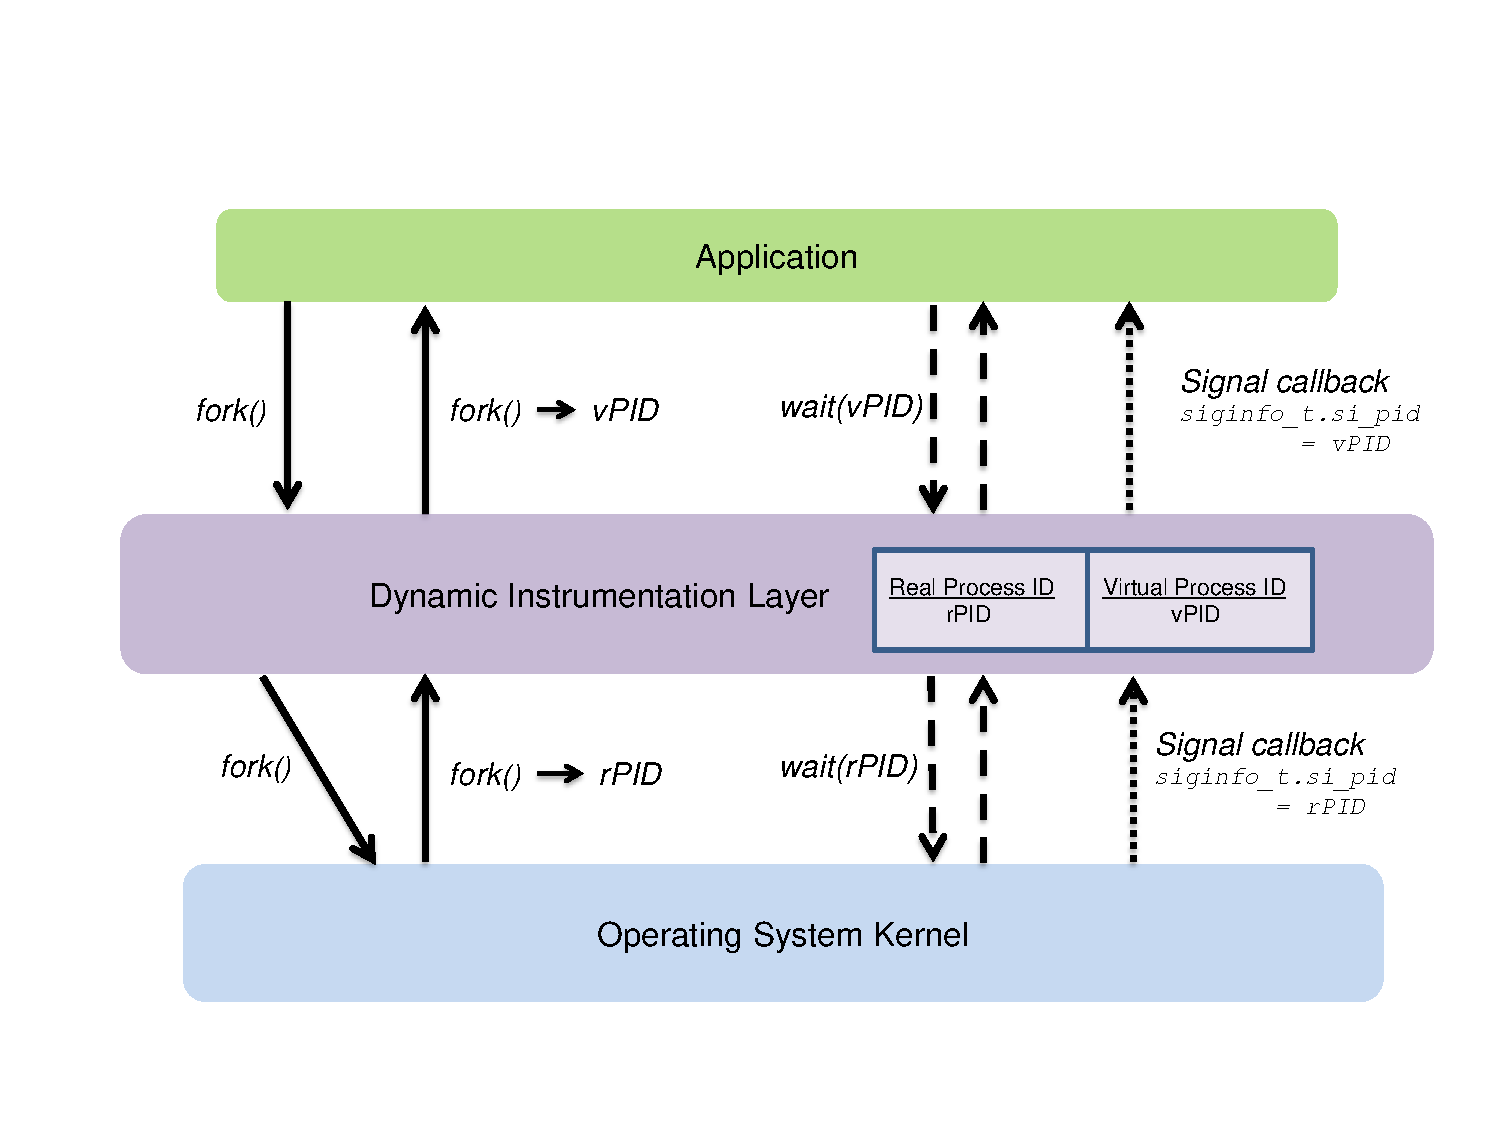
\includegraphics[trim=0cm 1cm 0cm 0.5cm, scale=0.60]{pid.pdf}
  \caption[Virtualizing the process ID layer using Pin]% 
  {All system calls and communications
  between the Linux user and kernel space are intercepted; 
  the dynamic instrumentation layer
  uses a PID translation table, and
  translates between real and virtual process IDs
  to ensure correctness. }
  
  \label{ch3:pidfig}
\end{figure} 

Using dynamic instrumentation, we can replace
real and unpredictable process IDs from kernel space
with virtual and unpredictable process IDs in user space.
As outlined in Section \ref{ch3:pid}, all interfaces
which use process IDs need to be carefully monitored
so that process IDs can be translated back and forth
for correctness. \newline

\noindent {\bf File I/O} \newline
Differences in input file contents across
executions would inevitably cause execution
to diverge, but overcoming nondeterminism arising
from time, randomization or process ID system calls
is typically sufficient to ensure that
file contents rarely differ in Linux services,
if at all. Some files that may differ
between two instances on start up (e.g. 
cache files or logs) can simply be 
deleted or replaced without sacrificing correctness.
Also, as mentioned already, \texttt{stat} 
timestamps are frequently not read, so
they can be replaced with fixed constants;
when they are read and only compared with other
\texttt{stat} timestamps, they can be replaced with 
ordinal numbers that perserve ordering;  
in all other cases, \texttt{stat} system calls 
can be faithfully replayed. \newline

\noindent{\bf Network I/O} \newline
The content of network configuration files
does not change in our experiments, so the strategies 
described to handle \texttt{stat} timestamps 
are sufficient for them. In the same vein, whenever an address is resolved
differently between execution instances because of DNS-based dynamic load balancing, 
we can intercept and replace resolved IPs with those
stored in the execution signature file.

If bytes read from sockets differ across different executions,
we need to understand the {\em context} to determine whether the
differences are serious (e.g. due to different requests)
or synthetic (e.g. due to timestamps). This can
can complicate design of the dynaminc instrumentation
layer because it 
may have to re-execute application or \texttt{libc}
logic to understand differences in raw bytes read from system calls.
We handle nondeterminism from \texttt{Netlink}
sockets in this way: the dynamic instrumentation layer 
re-executes \texttt{libc} logic associated
with understanding contents of \texttt{RTM\_NEWLINK}
messages to detect nondeterminsm from source/destination 
IDs, sequence numbers or interface statistics.
To handle variability in interface statistics,
we can simply overwrite them with fixed values.
This scheme can be generalized to handle
other kinds of network protocols as well.

As an alternative, we could
aggressively intercept Linux socket calls
and blindly replay them in all followers.
When many concurrent executions are reading data from the
same network source, this simulates the possibility
that all instances see the same results over the network
as the first instance. Such an approach, however,
can break correctness (Section \ref{ch3:issues}).
          
\newpage 
To overcome nondeterminism from ephemeral ports, 
we monitor the \texttt{bind} or \texttt{connect} 
system calls and change their arguments to explicitly request ports
in the ephemeral range rather than let the kernel 
assign them; if necessary,
we can also virtualize ephemeral ports
in a similar fashion to how we virtualize process IDs. \newline


\noindent{\bf Scalable I/O Schemes} \newline
To handle nondeterminism caused by unpredictable
ordering of I/O events,
we use techniques similar to those used 
for reordering signals,
as described by Figure \ref{ch3:reorderfig}.

\begin{figure}[h]
  \center
  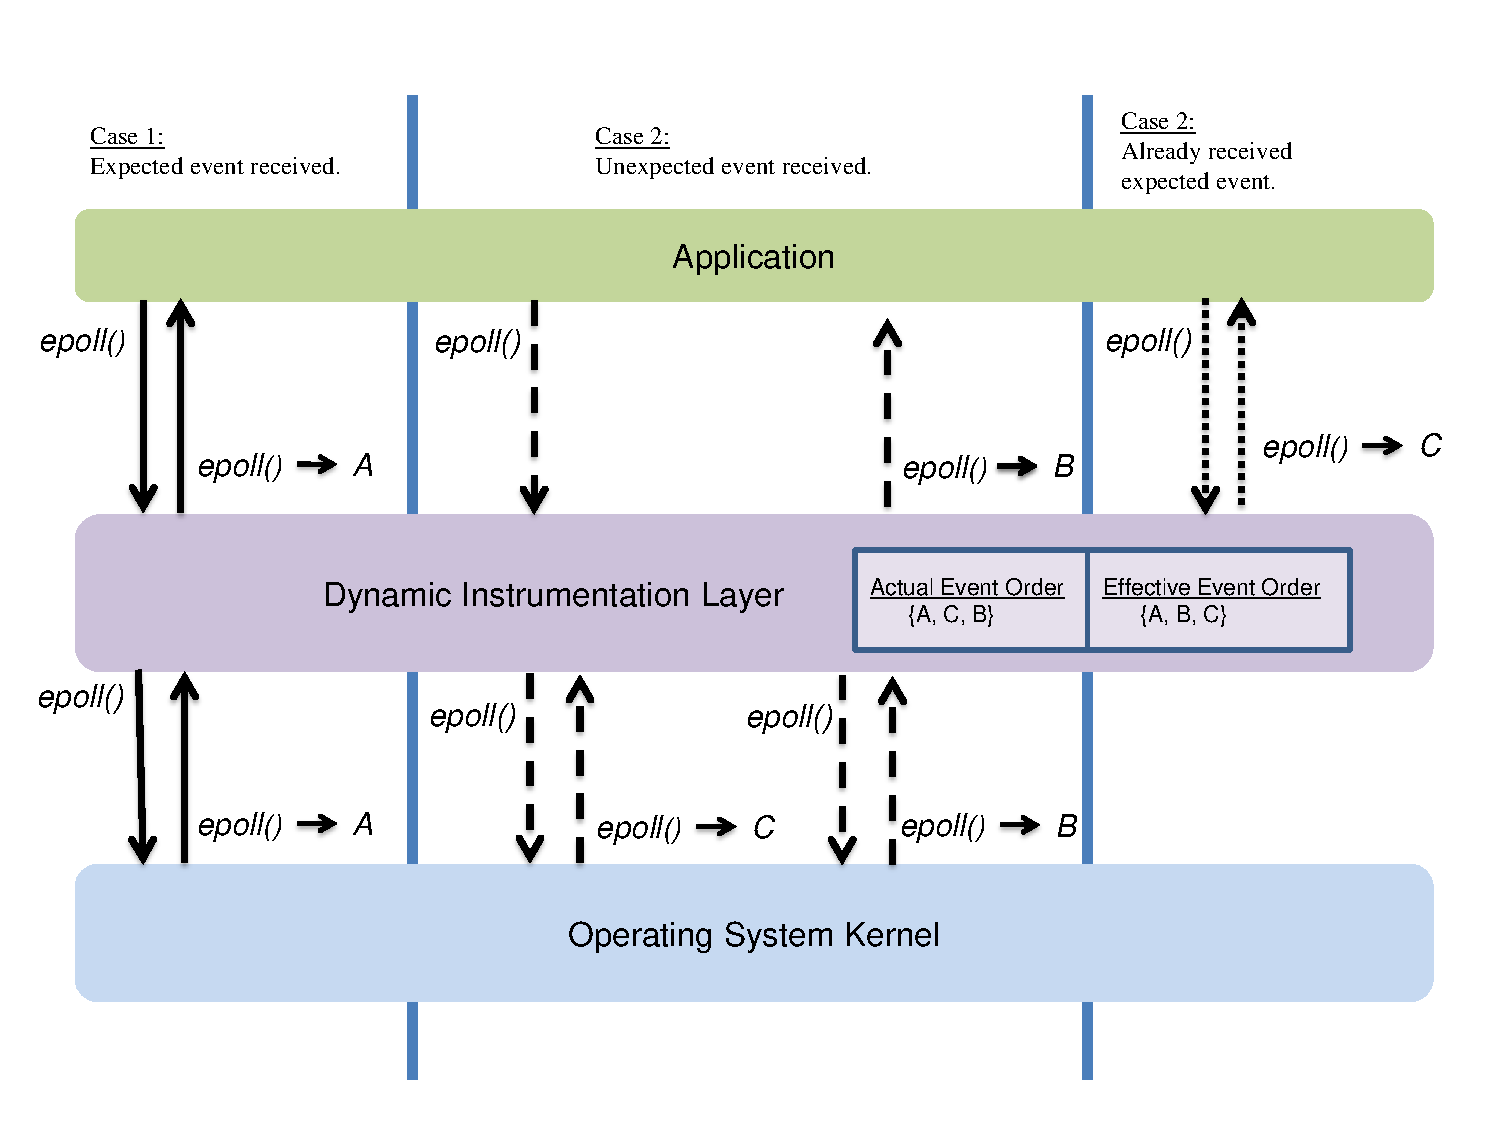
\includegraphics[trim=0cm 1.25cm 0cm 0.75cm, scale=0.60]{epoll.pdf}
  \caption[Reordering I/O events using Pin]% 
    {We intercept all \texttt{epoll} system calls,
    and use the execution signature file to
    achieve determinism. We do not ``replay'' I/O
    events because only events that actually do occur
    are delivered to the application instance. This
    diagram assumes \texttt{epoll} returns one event
    per call for the sake of illustration. }       
  \label{ch3:reorderfig}
\end{figure} 
              
Assuming that \texttt{epoll} returns just one event, figure
\ref{ch3:reorderfig} illustrates three possible cases that could occur:
\begin{itemize}
    \item The event returned by a call to \texttt{epoll} ($A$) is the one expected
    in the execution signature file ($A$). The instrumentation layer
    does not modify the system call.
    \item The desired event ($B$) has not been received yet,
    and \texttt{epoll} returns an unexpected event ($C$).
    The instrumentation layer stores the out-of-order event,
    and repeatedly calls \texttt{epoll} until the 
    the expected event is received.
    \item  A call to \texttt{epoll} is initiated, and the
    event desired ($C$) has already been received.
    The instrumentation layer does not 
    make a system call and simulates a return
    from \texttt{epoll} with the expected event instead.
\end{itemize}

Even if I/O events are reordered,
it is possible that different amounts
of data are available for ready
file descriptors across executions. We can 
mask this effect in the same
way we handle signals: if more bytes
are available (e.g. through \texttt{read}) 
than expected in the execution signature
file, we modify return values and \texttt{read}
buffers to delay the reading of these bytes
until the next \texttt{read}. In some corner
cases, we may have to ``fake'' readiness
in a call to \texttt{epoll}: if all bytes to be read from
a file descriptor have been read by 
the dynamic instrumentation layer (out of which
a few have not yet been delivered to the application),
there will be no more readiness events even
though the application expects them. If less-than-expected
bytes are available, we simply wait
till they are available by waiting for
another readiness update on the same file descriptor inside 
dynamic instrumentation layer.
In our experiments, this approach has been sufficient 
for overcoming nondeterminsm from event-based I/O
schemes.

For asynchronous I/O schemes (e.g. \texttt{aio\_read}), strategies
similar to those used for reordering
and precisely-timing signals would be necessary to hide
variable I/O latency and ordering.
\newline

\noindent {\bf Concurrency} \newline
Nondeterminism due to multi-threading
has been extensively documented; there
is a significant body of work that
attempts to overcome such nondeterminism
by using deterministic logical clocks
or record-and-replay approaches. 
For our experiments, we did not attempt to enforce
a total order on the instructions executed in multi-threaded
programs and just measured nondeterminism inside 
the main process for each Linux service.
To overcome nondeterminism caused
by multi-threading, we could incorporate
deterministic logical clocks 
into our design by augmenting the
execution signature file.

As mentioned before, a nondeterministic system scheduler
can cause variable timing of signals
or I/O events, which
can be handled using reordering and
timing strategies.
Work on deterministic
operating systems can
be extended to overcome this issue
in a more systematic manner. \newline

\noindent {\bf {\em Procfs}: The \texttt{`/proc/directory'}} \newline
Using the techniques described
already, I/O operations on {\em procfs} can be intercepted
and modified. We can 
replay reads from {\em procfs} using the execution signature
file if necessary or replace any statistics with fixed and 
reasonable values. The dynamic instrumentation layer 
must respect differences in virtual and real processes:
it must modify all \texttt{open} system calls with paths
of the form \texttt{`proc/[PID]'}
by switching real and virtual process IDs,
and a process must see its 
parent's virtual process ID when it reads
\texttt{`/proc/[PID]/status'}.

%\section{Results after Using Deterministic Execution} \label{ch3:data}
%We were able to achieve {\em fully} deterministic execution (i.e.
%user-mode execution traces that were 100\% identical) in several
%Linux services including \texttt{cron}, \texttt{ntp} and
%\texttt{cups} using these approaches.

%The next chapter describes the context in which nondeterminism
%occured in these services and the relative
%signficance of the various factors we have outline 
%as sources of nondeterminism in programs.







\section{Evaluation of Simulation} \label{sileval}
In order to evaluate the feasibility of this design,
we need to 
\section {Summary}
